\begin{frame}
\frametitle{Precision determination of the spin tune\,\textcolor{PineGreen}{\cite{PhysRevLett.115.094801}} II}

\vspace{-0.3cm}
\begin{columns}[c]
\column{0.46\textwidth}
\begin{block}{Precise time-stamping of events,}
\begin{itemize}
 \item allows us to monitor phase of measured asymmetry with (assumed) fixed spin tune $\nu_s$ in a $\SI{100}{s}$ cycle:
 \begin{equation}
 \begin{split}
    \nu_s(n) & = \nu_s^\text{fix} + \frac{1}{2\pi} \frac{\dd \tilde{\phi}}{\dd n}\\
             & = \nu_s^\text{fix} + \Delta \nu_s(n)
 \end{split}
 \end{equation}
\end{itemize}
\end{block}

\column{0.5\textwidth}
\begin{figure}
    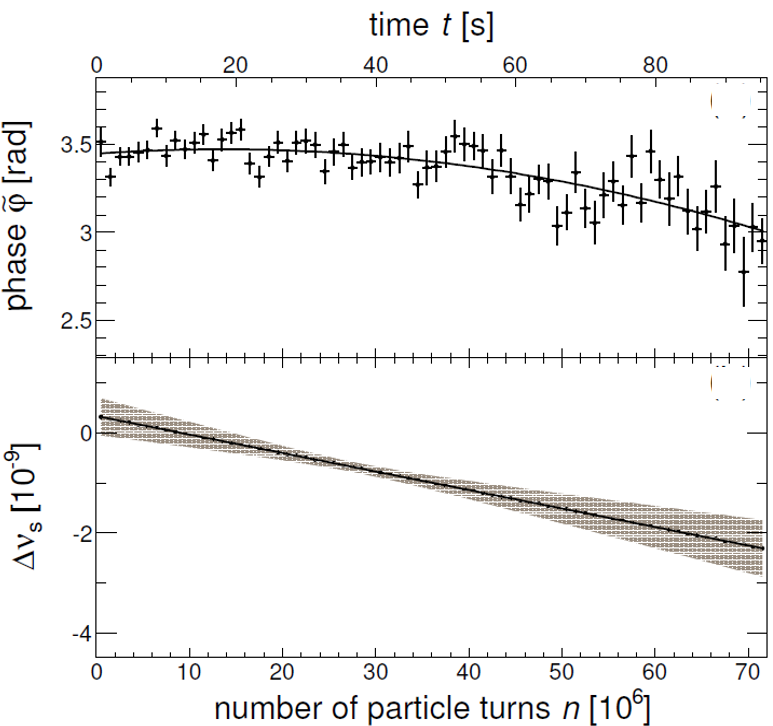
\includegraphics[width=0.9\textwidth]{spin-tune-determination.png}
\end{figure}
\end{columns}

\vspace{-0.2cm}
\begin{alertblock}{Experimental technique allows for:}
\begin{itemize}
 \item Spin tune $\nu_s$ determined to $\approx \num{e-8}$ in $\SI{2}{s}$ time interval.
 \item In a $\SI{100}{s}$ cycle at $t\approx \SI{38}{s}$, interpolated spin tune amounts to
            $|\nu_\text{s}| = (16097540628.3 \pm 9.7)\times 10^{-11}$, \textit{i.e.}, $\Delta \nu_s/\nu_s \approx \num{e-10}$.
 \item \textbf{$\Rightarrow$ new precision tool to study systematic effects in a storage ring.} 
\end{itemize}
\end{alertblock}

\end{frame}
